\documentclass[12pt,letterpaper]{article}
\usepackage{graphicx,textcomp}
\usepackage{natbib}
\usepackage{setspace}
\usepackage{fullpage}
\usepackage{color}
\usepackage[reqno]{amsmath}
\usepackage{amsthm}
\usepackage{fancyvrb}
\usepackage{amssymb,enumerate}
\usepackage[all]{xy}
\usepackage{endnotes}
\usepackage{lscape}
\newtheorem{com}{Comment}
\usepackage{float}
\usepackage{hyperref}
\newtheorem{lem} {Lemma}
\newtheorem{prop}{Proposition}
\newtheorem{thm}{Theorem}
\newtheorem{defn}{Definition}
\newtheorem{cor}{Corollary}
\newtheorem{obs}{Observation}
\usepackage[compact]{titlesec}
\usepackage{dcolumn}
\usepackage{tikz}
\usetikzlibrary{arrows}
\usepackage{multirow}
\usepackage{xcolor}
\newcolumntype{.}{D{.}{.}{-1}}
\newcolumntype{d}[1]{D{.}{.}{#1}}
\definecolor{light-gray}{gray}{0.65}
\usepackage{url}
\usepackage{listings}
\usepackage{color}

\definecolor{codegreen}{rgb}{0,0.6,0}
\definecolor{codegray}{rgb}{0.5,0.5,0.5}
\definecolor{codepurple}{rgb}{0.58,0,0.82}
\definecolor{backcolour}{rgb}{0.95,0.95,0.92}

\lstdefinestyle{mystyle}{
	backgroundcolor=\color{backcolour},   
	commentstyle=\color{codegreen},
	keywordstyle=\color{magenta},
	numberstyle=\tiny\color{codegray},
	stringstyle=\color{codepurple},
	basicstyle=\footnotesize,
	breakatwhitespace=false,         
	breaklines=true,                 
	captionpos=b,                    
	keepspaces=true,                 
	numbers=left,                    
	numbersep=5pt,                  
	showspaces=false,                
	showstringspaces=false,
	showtabs=false,                  
	tabsize=2
}
\lstset{style=mystyle}
\newcommand{\Sref}[1]{Section~\ref{#1}}
\newtheorem{hyp}{Hypothesis}

\title{Problem Set 3}
\date{Due: November 12, 2026}
\author{
	Applied Stats/Quant Methods 1\\
	Kanon Saito
}

\begin{document}
	\maketitle
	\section*{Instructions}
	\begin{itemize}
		\item Please show your work! You may lose points by simply writing in the answer. If the problem requires you to execute commands in \texttt{R}, please include the code you used to get your answers. Please also include the \texttt{.R} file that contains your code. If you are not sure if work needs to be shown for a particular problem, please ask.
	\item Your homework should be submitted electronically on GitHub.
	\item This problem set is due before 23:59 on Thursday November 12, 2026. No late assignments will be accepted.

	\end{itemize}

		\vspace{.25cm}
	
\noindent In this problem set, you will run several regressions and create an add variable plot (see the lecture slides) in \texttt{R} using the \texttt{incumbents\_subset.csv} dataset. Include all of your code.

	\vspace{.5cm}
\section*{Question 1}
\vspace{.25cm}
\noindent We are interested in knowing how the difference in campaign spending between incumbent and challenger affects the incumbent's vote share. 
	\begin{enumerate}
		\item Run a regression where the outcome variable is \texttt{voteshare} and the explanatory variable is \texttt{difflog}. \vspace{.5cm}\newline 
		R:
		\lstinputlisting[linerange=35-36]{PS03_answers_KS.R}\vspace{.5cm}
		\begin{verbatim}
			Call:
			lm(formula = voteshare ~ difflog, data = inc.sub)
			
			Residuals:
			Min       1Q   Median       3Q      Max 
			-0.26832 -0.05345 -0.00377  0.04780  0.32749 
			
			Coefficients:
			Estimate Std. Error t value Pr(>|t|)    
			(Intercept) 0.579031   0.002251  257.19   <2e-16 ***
			difflog     0.041666   0.000968   43.04   <2e-16 ***
			---
			Signif. codes:  0 ‘***’ 0.001 ‘**’ 0.01 ‘*’ 0.05 ‘.’ 0.1 ‘ ’ 1
			
			Residual standard error: 0.07867 on 3191 degrees of freedom
			Multiple R-squared:  0.3673,	Adjusted R-squared:  0.3671 
			F-statistic:  1853 on 1 and 3191 DF,  p-value: < 2.2e-16
		\end{verbatim}
		On average, a one-unit increase in the difference in campaign spending (difflog) is associated with a 0.0417-unit increase in the incumbent's vote share.
		When there is no difference in campaign spending (difflog = 0), the predicted vote share for the incumbent is 0.5790 (57.9\%).
		\vspace{.5cm}
		\item Make a scatterplot of the two variables and add the regression line. 
		
		R: 
		\lstinputlisting[linerange=38-46]{PS03_answers_KS.R}
		Figure 1 (scatterplot)
		\begin{figure}[H]
			\centering
			\vspace{.5cm}
			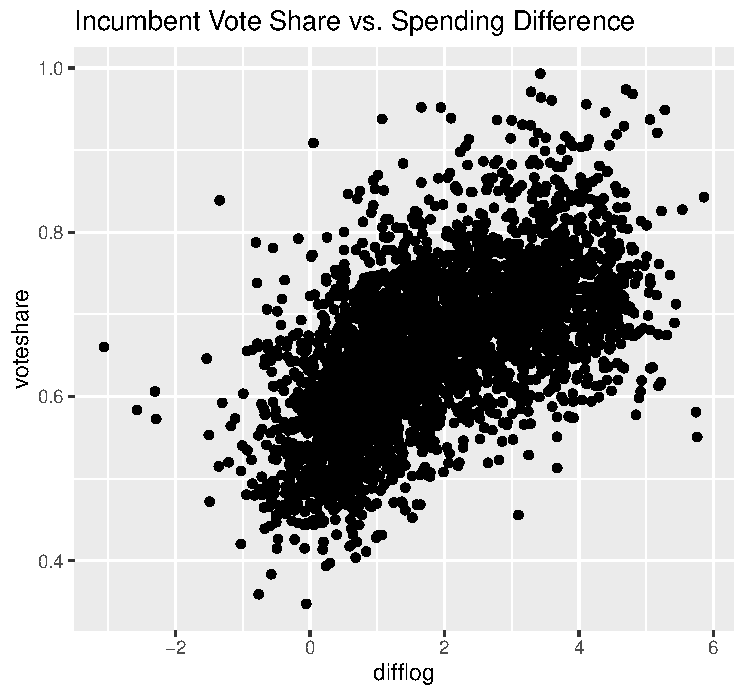
\includegraphics[width=8cm]{Q1-1.pdf}
		\end{figure}
		Figure 2 (scatterplot + regression line)
		\begin{figure}[H]
			\centering
			\vspace{.5cm}
			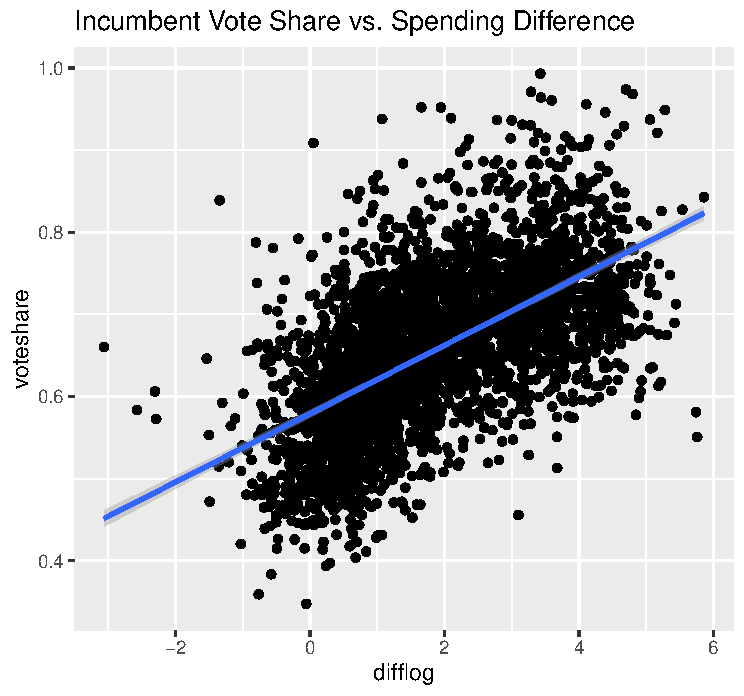
\includegraphics[width=8cm]{Q1-2.pdf}
		\end{figure}
		This scatterplot displays the positive relationship between the difference in campaign spending and the incumbent voteshare.
		The data points lie relatively close to the regression line, suggesting a strong linear relationship between the two variables.
		\newpage
	\item Save the residuals of the model in a separate object.	\\
	
	R: 
	\lstinputlisting[linerange=48-49]{PS03_answers_KS.R}
	\begin{verbatim}
	            1             2             3             4             5             6 
	-0.0004227622 -0.0316840149 -0.0045514943  0.0386688767  0.0355287965  0.0322832521 
	\end{verbatim}
	
	The residuals represent the variation in the voteshare that is unexplained by the difflog (we remove the effect of difflog from the voteshare variable).
	
	\item Write the prediction equation.
	\vspace{.5cm}
	
	$\widehat{\text{voteshare}} = 0.5790 + 0.0417 \times \text{difflog}$
	\end{enumerate}
	\vspace{2cm}

\section*{Question 2}
\noindent We are interested in knowing how the difference between incumbent and challenger's spending and the vote share of the presidential candidate of the incumbent's party are related.	\vspace{.25cm}
	\begin{enumerate}
		\item Run a regression where the outcome variable is \texttt{presvote} and the explanatory variable is \texttt{difflog}.\\
		
		R:
		\lstinputlisting[linerange=54-55]{PS03_answers_KS.R}
		\begin{verbatim}
		Call:
		lm(formula = presvote ~ difflog, data = inc.sub)
		
		Residuals:
		Min       1Q   Median       3Q      Max 
		-0.32196 -0.07407 -0.00102  0.07151  0.42743 
		
		Coefficients:
		Estimate Std. Error t value Pr(>|t|)    
		(Intercept) 0.507583   0.003161  160.60   <2e-16 ***
		difflog     0.023837   0.001359   17.54   <2e-16 ***
		---
		Signif. codes:  0 ‘***’ 0.001 ‘**’ 0.01 ‘*’ 0.05 ‘.’ 0.1 ‘ ’ 1
		
		Residual standard error: 0.1104 on 3191 degrees of freedom
		Multiple R-squared:  0.08795,	Adjusted R-squared:  0.08767 
		F-statistic: 307.7 on 1 and 3191 DF,  p-value: < 2.2e-16
		\end{verbatim}
		On average, a one-unit increase in the difference in campaign spending (difflog) is associated with a 0.0238-unit increase in the vote share of the presidential candidate of the incumbent's party.
		When there is no difference in campaign spending (difflog = 0), the predicted vote share for the presidential candidate of the incumbent's party is 0.5076 (50.8\%).
		\vspace{.5cm}
		\item Make a scatterplot of the two variables and add the regression line. \\
		
		R:
		\lstinputlisting[linerange=57-64]{PS03_answers_KS.R}
		Figure 3 (scatterplot)
		\begin{figure}[H]
			\centering
			\vspace{.5cm}
			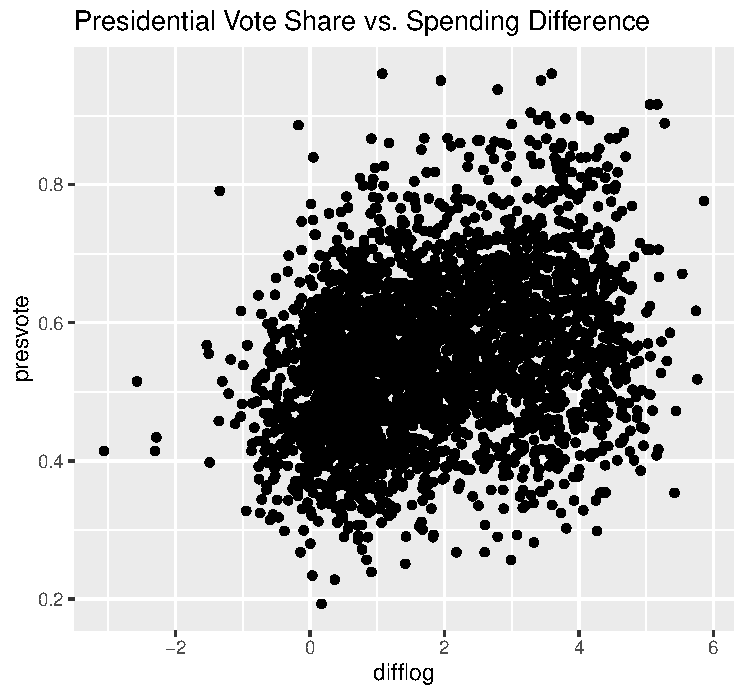
\includegraphics[width=8cm]{Q2-1.pdf}
		\end{figure}
		Figure 4 (scatterplot + regression line)
		\begin{figure}[H]
			\centering
			\vspace{.5cm}
			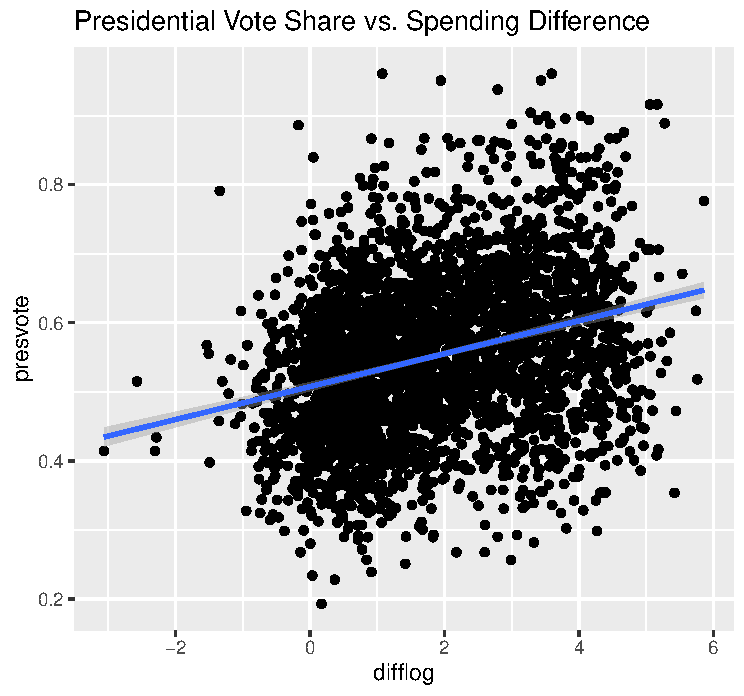
\includegraphics[width=8cm]{Q2-2.pdf}
		\end{figure}
		This scatterplot displays the positive relationship between the difference in campaign spending and the vote share of the presidential candidate of the incumbent's party.
		The data points show some dispersion around the regression line, suggesting a relatively weak model fit.
		\item Save the residuals of the model in a separate object.	\\
		
		R: 
		\lstinputlisting[linerange=66-67]{PS03_answers_KS.R}
		\begin{verbatim}
		           1            2            3            4            5            6 
		0.005605594  0.037578519 -0.053134788 -0.052993694 -0.045842994  0.074339701 
		\end{verbatim}
		The residuals represent the variation in the presidential voteshare that is unexplained by the difflog (we remove the effect of difflog from the voteshare variable).
		\vspace{.5cm}
		\item Write the prediction equation.\\
		
		$\widehat{\text{presvote}} = 0.5076 + 0.0238 \times \text{difflog}$
	\end{enumerate}
	
	\vspace{.5cm}
\section*{Question 3}

\noindent We are interested in knowing how the vote share of the presidential candidate of the incumbent's party is associated with the incumbent's electoral success.
	\vspace{.25cm}
	\begin{enumerate}
		\item Run a regression where the outcome variable is \texttt{voteshare} and the explanatory variable is \texttt{presvote}.\\
		
		R:
		\lstinputlisting[linerange=71-72]{PS03_answers_KS.R}
		\begin{verbatim}
		Call:
		lm(formula = voteshare ~ presvote, data = inc.sub)
		
		Residuals:
		Min       1Q   Median       3Q      Max 
		-0.27330 -0.05888  0.00394  0.06148  0.41365 
		
		Coefficients:
		Estimate Std. Error t value Pr(>|t|)    
		(Intercept) 0.441330   0.007599   58.08   <2e-16 ***
		presvote    0.388018   0.013493   28.76   <2e-16 ***
		---
		Signif. codes:  0 ‘***’ 0.001 ‘**’ 0.01 ‘*’ 0.05 ‘.’ 0.1 ‘ ’ 1
		
		Residual standard error: 0.08815 on 3191 degrees of freedom
		Multiple R-squared:  0.2058,	Adjusted R-squared:  0.2056 
		F-statistic:   827 on 1 and 3191 DF,  p-value: < 2.2e-16
		\end{verbatim}
		On average, a one-unit increase in the vote share of the presidential candidate of the incumbent's party (presvote) is associated with a 0.3880-unit increase in the incumbent voteshare.
		When the vote share of the presidential candidate of the incumbent's party is zero (presvote = 0), the predicted incumbent's vote share is 0.4413 (44.1\%).
		\vspace{.5cm}
		\item Make a scatterplot of the two variables and add the regression line. \\
		R:
		\lstinputlisting[linerange=74-81]{PS03_answers_KS.R}
		Figure 5 (scatterplot)
		\begin{figure}[H]
			\centering
			\vspace{.5cm}
			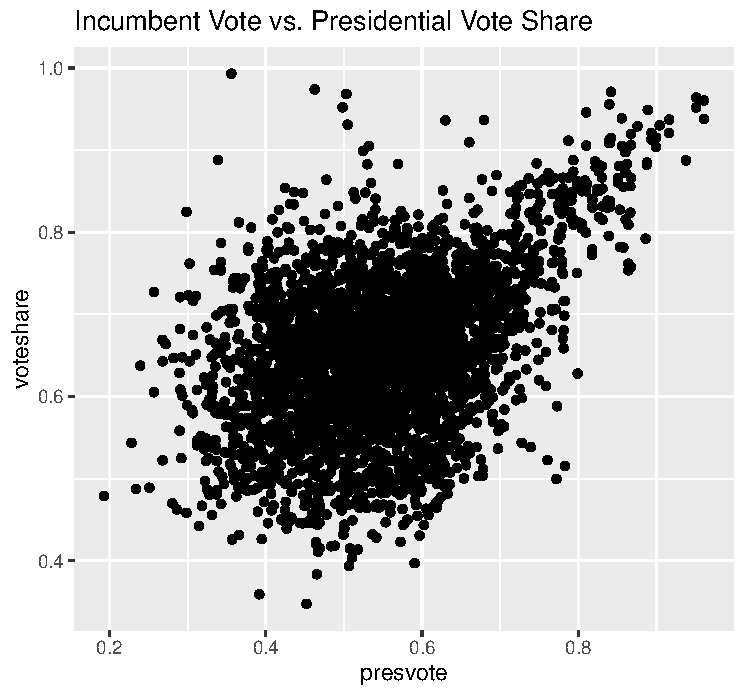
\includegraphics[width=8cm]{Q3-1.pdf}
		\end{figure}
		Figure 6 (scatterplot + regression line)
		\begin{figure}[H]
			\centering
			\vspace{.5cm}
			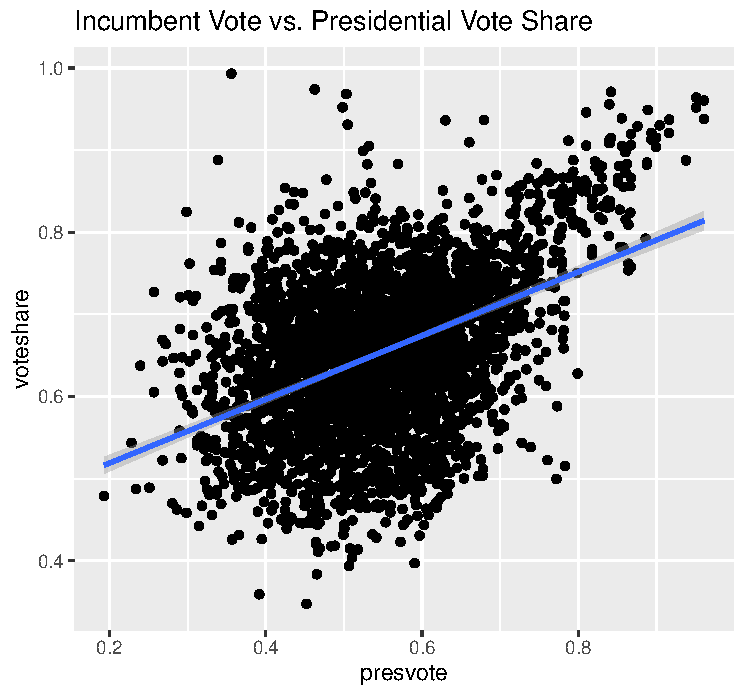
\includegraphics[width=8cm]{Q3-2.pdf}
		\end{figure}
		This scatterplot displays the positive relationship between the vote share of the presidential candidate of the incumbent's party and the incumbent voteshare.
		The data points show some dispersion around the regression line, suggesting a relatively weak model fit.
			\vspace{.5cm}
		\item Write the prediction equation.\\
		
		$\widehat{\text{voteshare}} = 0.4413 + 0.3880 \times \text{presvote}$
		
	\end{enumerate}
	\vspace{.5cm}
\section*{Question 4}
\noindent The residuals from part (a) tell us how much of the variation in \texttt{voteshare} is $not$ explained by the difference in spending between incumbent and challenger. The residuals in part (b) tell us how much of the variation in \texttt{presvote} is $not$ explained by the difference in spending between incumbent and challenger in the district.
	\begin{enumerate}
		\item Run a regression where the outcome variable is the residuals from Question 1 and the explanatory variable is the residuals from Question 2.	\\
		
		R:
		\lstinputlisting[linerange=85-86]{PS03_answers_KS.R}
		\begin{verbatim}
		Call:
		lm(formula = res1 ~ res2)
		
		Residuals:
		Min       1Q   Median       3Q      Max 
		-0.25928 -0.04737 -0.00121  0.04618  0.33126 
		
		Coefficients:
		Estimate Std. Error t value Pr(>|t|)    
		(Intercept) -1.942e-18  1.299e-03    0.00        1    
		res2         2.569e-01  1.176e-02   21.84   <2e-16 ***
		---
		Signif. codes:  0 ‘***’ 0.001 ‘**’ 0.01 ‘*’ 0.05 ‘.’ 0.1 ‘ ’ 1
		
		Residual standard error: 0.07338 on 3191 degrees of freedom
		Multiple R-squared:   0.13,	Adjusted R-squared:  0.1298 
		F-statistic:   477 on 1 and 3191 DF,  p-value: < 2.2e-16
		\end{verbatim}
		On average, a one-unit increase in the variation of voteshare unexplained by campaign spending difference (res2) is associated with a 0.2569-unit increase in the variation of presvote unexplained by campaign spending difference (res1).
		When the residual of voteshare unexplained by difflog is zero (res2 = 0), the predicted residual of presvote is approximately 0 ($-1.942 \times 10^{-18}$).
		\vspace{.5cm}
		\item Make a scatterplot of the two residuals and add the regression line. \\
		
		R:
		\lstinputlisting[linerange=88-95]{PS03_answers_KS.R}
		Figure 7 (scatterplot)
		\begin{figure}[H]
			\centering
			\vspace{.5cm}
			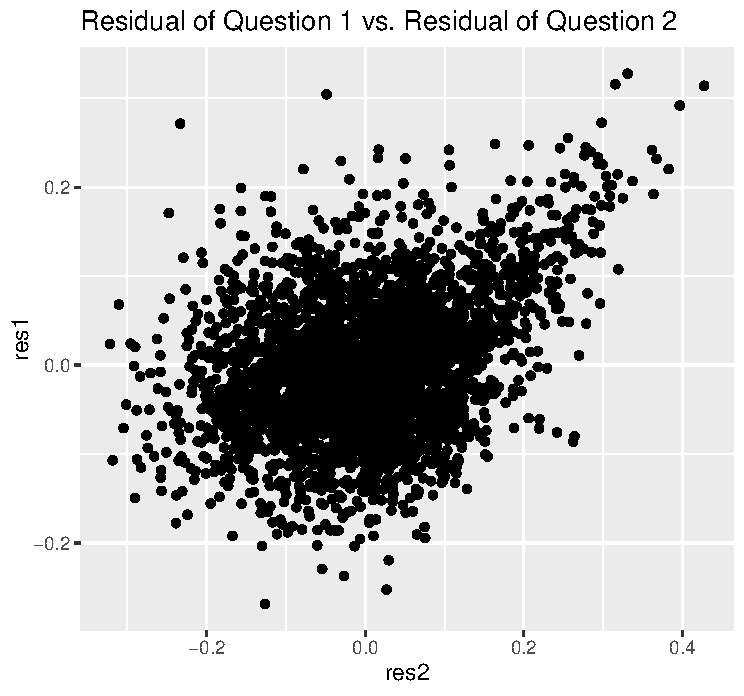
\includegraphics[width=7.5cm]{Q4-1.pdf}
		\end{figure}
		Figure 8 (scatterplot + regression line)
		\begin{figure}[H]
			\centering
			\vspace{.5cm}
			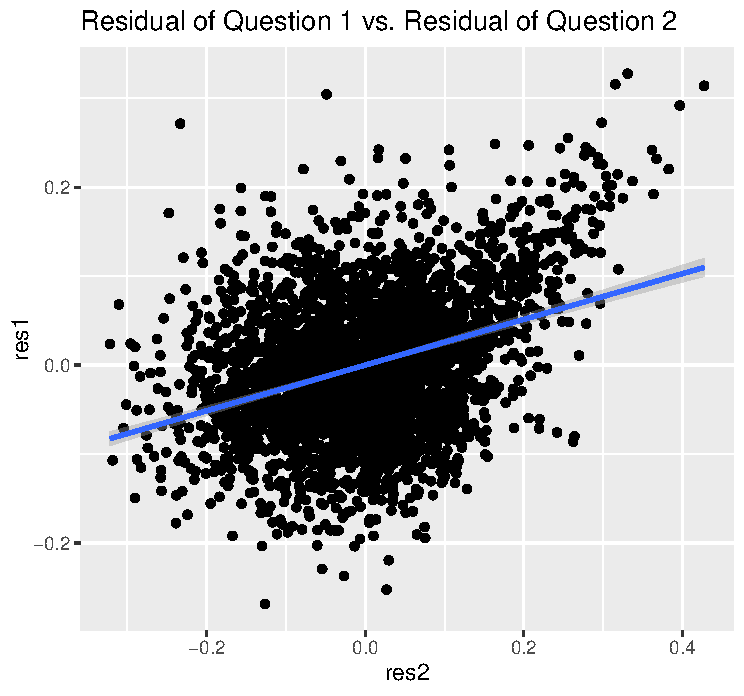
\includegraphics[width=7.5cm]{Q4-2.pdf}
		\end{figure}
		This scatterplot displays the positive relationship between the variation of voteshare unexplained by campaign spending difference (res2) and the variation of presvote unexplained by campaign spending difference (res1).
		The data points show some dispersion around the regression line, suggesting a relatively weak model fit.
		\vspace{.5cm}
		\item Write the prediction equation.
		
		$\widehat{\text{res1}} =  0.2569 \times \text{res2}$
		
		The intercept is calculated as $-1.942 \times 10^{-18}$, which is essentially zero. 
	\end{enumerate}
	
	\vspace{.5cm}

\section*{Question 5}
\noindent What if the incumbent's vote share is affected by both the president's popularity and the difference in spending between incumbent and challenger? 
	\begin{enumerate}
		\item Run a regression where the outcome variable is the incumbent's \texttt{voteshare} and the explanatory variables are \texttt{difflog} and \texttt{presvote}.	\\
		
		R:
		\lstinputlisting[linerange=100-101]{PS03_answers_KS.R}
		\begin{verbatim}
		Call:
		lm(formula = voteshare ~ difflog + presvote, data = inc.sub)
		
		Residuals:
		Min       1Q   Median       3Q      Max 
		-0.25928 -0.04737 -0.00121  0.04618  0.33126 
		
		Coefficients:
		Estimate Std. Error t value Pr(>|t|)    
		(Intercept) 0.4486442  0.0063297   70.88   <2e-16 ***
		difflog     0.0355431  0.0009455   37.59   <2e-16 ***
		presvote    0.2568770  0.0117637   21.84   <2e-16 ***
		---
		Signif. codes:  0 ‘***’ 0.001 ‘**’ 0.01 ‘*’ 0.05 ‘.’ 0.1 ‘ ’ 1
		
		Residual standard error: 0.07339 on 3190 degrees of freedom
		Multiple R-squared:  0.4496,	Adjusted R-squared:  0.4493 
		F-statistic:  1303 on 2 and 3190 DF,  p-value: < 2.2e-16
		\end{verbatim}

		On average, a one-unit increase in the difference in campaign spending (difflog) is associated with a 0.0355-unit increase in the incumbent's vote share, holding the presidential vote share constant. In addition, on average, a one-unit increase in the presidential vote share (presvote) is associated with a 0.2569-unit increase in the incumbent's vote share, holding the difference in campaign spending constant.
		When there is no difference in campaign spending (difflog = 0) and the presidential vote share is 0\%, the predicted incumbent's vote share is 0.4486 (44.9\%).
		\vspace{.5cm}
		\item Write the prediction equation.\\
		
		$\widehat{\text{voteshare}} = 0.4486 + 0.0355 \times \text{difflog} + 0.2569 \times \text{presvote}$
		
		
		\item What is it in this output that is identical to the output in Question 4? Why do you think this is the case?
		 \vspace{1cm}
		The regression coefficient and SE of the two residuals in Q4 and the regression coefficient and SE of presvote in Q5 are exactly the same.
		In Q1, the residuals represent the part of voteshare unexplained by difflog (we remove the effect of difflog from the voteshare variable). Similarly, in Q2, the residuals represent the part of presvote unexplained by difflog (we remove the effect of difflog from the presvote variable). Therefore, in Q4, we regress the Q1 residuals on the Q2 residuals. This allows us to control for the effect of difflog by removing it from both variables, leaving only the effect of presvote on voteshare. This results in a coefficient of 0.2569 and an SE of 0.01176.\newline
		\begin{verbatim}
			Coefficients:
			Estimate Std. Error t value Pr(>|t|)    
			(Intercept) -1.942e-18  1.299e-03    0.00        1    
			res2         2.569e-01  1.176e-02   21.84   <2e-16 ***
		\end{verbatim}
		On the other hand, the multiple regression model in Q5 gives exactly the same results. Since multiple regression coefficients can statistically control for the effects of other variables in the model, the regression coefficient of presvote in Q5 represents its effect on voteshare independent of difflog. This results in the exact same coefficient of 0.2569 (0.2568770) and SE of 0.01176.\newline
		\begin{verbatim}
			Coefficients:
			Estimate Std. Error t value Pr(>|t|)    
			(Intercept) 0.4486442  0.0063297   70.88   <2e-16 ***
			difflog     0.0355431  0.0009455   37.59   <2e-16 ***
			presvote    0.2568770  0.0117637   21.84   <2e-16 ***
		\end{verbatim}
	\end{enumerate}




\end{document}
